\documentclass[12pt, letterpaper]{article}

\usepackage[utf8]{inputenc}
\usepackage[margin=1in]{geometry}
\usepackage{titlesec}
\usepackage{enumitem}
\usepackage{booktabs}
\usepackage{array}
\usepackage{xcolor}
\usepackage{hyperref}
\usepackage{setspace}
\usepackage{graphicx}
\usepackage{tikz}

\definecolor{darkblue}{RGB}{44, 62, 80}
\definecolor{mediumblue}{RGB}{52, 73, 94}
\definecolor{accentred}{RGB}{192, 57, 43}

\titleformat{\section}
{\Large\bfseries\color{darkblue}}
{\thesection}{1em}{}

\titleformat{\subsection}
{\large\bfseries\color{mediumblue}}
{\thesubsection}{1em}{}

\hypersetup{
    colorlinks=true,
    linkcolor=darkblue,
    urlcolor=darkblue
}

\setlength{\parskip}{0.8em}
\setlength{\parindent}{0pt}

\begin{document}

% Title
\begin{center}
    {\Huge\bfseries\color{darkblue} THE ORDER}

    \vspace{0.3cm}

    {\Large\itshape A First-Person Psychological Horror Survival Game}

    \vspace{1cm}

    {\large Project Proposal (Deliverable 1)}

    \vspace{0.5cm}

    {\large Karl Seryani, Kirill Delyukin, Raghav Gulati}

    \vspace{0.3cm}

    {\large CS 4483B: Game Design}

    {\large February 11, 2026}
\end{center}

\vspace{0.8cm}

%===================================================================
\section{Conceptual Framework}
%===================================================================

\subsection{Theme and Narrative}

The Order explores guilt, sacrifice, and the fragility of memory through the story of two brothers destroyed by one unforgivable act.

\textbf{Backstory:} John and Mike are brothers who served together in a covert military unit called The Order. During their service, John stole nuclear launch codes and sold them. The codes were used. Bombs fell. Cities were destroyed. Millions died. When Mike discovered that his own brother was responsible, he made a choice: rather than turn John in, Mike took the blame. He was court-martialed, imprisoned, and tortured for years for a crime he did not commit. John, caught in the blast radius of the very destruction he caused, was critically injured and fell into a coma. He was placed in a secure military bunker where he remained unconscious for years. While Mike endured torture in a cell, John slept through the consequences of what he had done.

Eventually Mike was released, broken and changed. He found John still comatose in the bunker. He could have killed John in his sleep, but that would have been too easy. John would never have to know what he did. So Mike waited. He scattered clues throughout the facility: classified documents detailing the stolen codes, photographs of the brothers before the war, recordings from Mike's trial, evidence of the devastation. Then he locked the exits and began patrolling the halls.

\textbf{The Game:} John wakes from his coma with no memory. The brain damage from the blast wiped everything clean. He is alone in a dark bunker with only a flashlight, hunted by a violent man he does not recognize. Through 17 scattered clues (documents, photographs, recordings), the player pieces together the truth: the hunter is John's brother, and it was John who destroyed the world. Mike does not hunt John to kill him. He hunts John to force him to feel hunted, afraid, and powerless, a fraction of what Mike endured for years. The clues are Mike's real weapon. He wants John to find them, to understand what he did and what Mike sacrificed. The horror is not the man chasing you. The horror is you.

\textbf{Prologue:} The game opens with a brief prologue set in a country house. The player controls John moments after launching the nuclear strike. The scene is scripted: as soon as John steps outside and descends the front stairs, the blast wave hits. The screen flashes white, then cuts to black. The title, ``THE ORDER,'' fades onto the screen and lingers before fading out. The game then cuts to John waking up on a bed inside the bunker, years later, with no memory. He stands, and gameplay begins.

\subsection{Target Audience and Genre}

\textbf{Target Audience:} Mature players (18+) who enjoy narrative-driven horror with psychological depth. Fans of Outlast, Amnesia: The Dark Descent, SOMA, and Silent Hill. The game also appeals to players who enjoy discovery-based narratives like Gone Home and Firewatch, wrapped in a survival horror framework.

\textbf{Genre:} First-person psychological horror survival with stealth and exploration. The first-person perspective places the player directly in John's body: you see only what the flashlight reveals, hear Mike's footsteps through corridors, and must decide in real time whether to run, hide, or press forward.

\subsection{Engagement Strategy}

The Order engages players through four pillars:
\begin{itemize}[leftmargin=2em, topsep=0pt, itemsep=2pt]
    \item \textbf{Tension and Vulnerability:} Mike patrols while John's sanity drains. The flashlight is essential but reveals John's position. Every action is a calculated risk.
    \item \textbf{Mystery and Discovery:} Neither John nor the player knows the truth. Each clue rewards exploration with narrative revelations building toward an emotional climax, delivered through environmental storytelling at the player's own pace.
    \item \textbf{Meaningful Choice:} Nine endings depend on which clues John finds and what he chooses at the exit. No ending is ``game over''; every ending is narratively intentional.
    \item \textbf{Mastery Through Knowledge:} Replaying rewards map knowledge and strategic awareness, not power upgrades. Players learn patrol routes and clue locations to optimize runs for specific endings.
\end{itemize}

%===================================================================
\section{Design Principles}
%===================================================================

\subsection{MDA Framework}

\textbf{Mechanics:} First-person movement with stamina (walk, sprint, crouch); flashlight as visibility tool that also exposes the player; sanity meter with passive drain and event-based acceleration; 17 clues across three categories (Truth, Mike, Weapon); hunter AI with finite state machine (patrol, investigate, chase, search); interactive doors; hiding spots with breath-holding minigame.

\textbf{Dynamics:} Risk-reward exploration (more clues means better endings but more danger); flashlight dilemma (necessary for navigation but doubles detection range); sound-based stealth (sprinting draws Mike, crouching is slow but silent); sanity death spiral (low sanity reduces stamina, making escape harder); route optimization on replays.

\textbf{Aesthetics} (LeBlanc's taxonomy): \textit{Sensation} through oppressive darkness and spatial audio; \textit{Challenge} through dual pressure of hunter and sanity; \textit{Discovery} through 17 clues and environmental storytelling; \textit{Narrative} through an emotionally devastating story of brotherhood and guilt; \textit{Submission} through first-person immersion and minimal HUD.

\subsection{Bartle's Player Types}

\begin{table}[h]
\centering
\small
\begin{tabular}{@{}p{2.5cm}p{5cm}p{5cm}@{}}
\toprule
\textbf{Type} & \textbf{Appeal} & \textbf{Design Elements} \\
\midrule
Explorers & Finding all 17 clues, uncovering hidden rooms, learning patrol routes & Environmental storytelling, 3-floor bunker, camera terminals \\
\addlinespace
Achievers & Unlocking all 9 endings, mastering efficient runs & Ending tracking, knowledge-gated true ending \\
\addlinespace
Killers & Finding the weapon and confronting Mike directly & Weapon clue, combat ending (framed as morally worst) \\
\addlinespace
Socializers & Debating endings and theories about the brothers & Complex narrative encourages post-game discussion \\
\bottomrule
\end{tabular}
\end{table}

%===================================================================
\section{Ideation and Brainstorming}
%===================================================================

\subsection{Process and Theme Evolution}

The design began with analysis of team preferences: narrative-driven games (The Last of Us, SOMA), vulnerability-based horror (Outlast, Amnesia), and knowledge-gated progression over grind-based advancement.

Three concepts were developed: (1) \textbf{Depths}, a descending survival game, rejected for being narratively shallow; (2) \textbf{The Chase}, a pursuit-horror game with discovery mechanics, selected for its alignment of tension and narrative; (3) \textbf{Last Run}, a roguelike with environmental storytelling, rejected because procedural generation conflicts with hand-crafted narrative.

The chase concept evolved through four iterations: generic monster pursuit, then a human serial killer antagonist, then the hunter as the player's brother with a war crime backstory, and finally the current direction where John is the true villain who stole nuclear launch codes and Mike is the tragic figure who sacrificed everything to protect him. The original design was top-down 2D, but the team shifted to first-person 3D for immersion, visibility constraints, spatial audio impact, environmental storytelling, and genre alignment with influences like Outlast and Amnesia.

\subsection{Goals}

\begin{itemize}[leftmargin=2em, topsep=0pt, itemsep=2pt]
    \item Create sustained tension through dual pressure: Mike (external) and sanity (internal)
    \item Reward knowledge over time investment; a skilled player completes the game in 15 minutes, a first-timer in 45
    \item Deliver narrative where understanding depends on willingness to take risks
    \item Support replayability through nine endings with distinct narrative resolutions
\end{itemize}

%===================================================================
\section{Core Mechanics and Gameplay}
%===================================================================

\subsection{Core Loop}

The moment-to-moment loop repeats every 15 to 60 seconds: (1) \textbf{Listen} for Mike's footsteps via spatial audio; (2) \textbf{Scout} with the flashlight; (3) \textbf{Move} through the bunker (walk quietly or sprint loudly); (4) \textbf{Search} rooms for clues; (5) \textbf{React} to Mike (hide, sprint, or freeze); (6) \textbf{Recover} sanity and stamina. The meta loop across sessions rewards map knowledge, route optimization, and ending collection.

\subsection{Ending System}

Nine endings are determined by two axes: \textbf{knowledge} (clues collected) and \textbf{choice} (action at the exit). Three choices are available: use the weapon, confront Mike, or flee. Combined with low, medium, or high knowledge, these produce nine outcomes ranging from ``Blind Violence'' (killing Mike in total ignorance, the darkest ending) to ``Absolution'' (confronting Mike with full understanding of both the crime and the sacrifice, the true ending where Mike forgives John and they walk out together).

\begin{table}[h]
\centering
\small
\renewcommand{\arraystretch}{1.4}
\begin{tabular}{@{}p{2cm}|p{3.5cm}|p{3.5cm}|p{3.5cm}@{}}
\toprule
& \textbf{Use Weapon} & \textbf{Confront Mike} & \textbf{Flee} \\
\midrule
\textbf{Low} \newline (0--5 clues) & \textcolor{accentred}{Blind Violence} \newline Kills Mike in ignorance & Confused Rage \newline Screams at a stranger & Hollow Escape \newline Runs with no understanding \\
\midrule
\textbf{Medium} \newline (6--11 clues) & Guilty Execution \newline Kills knowing it is his brother & Bitter Standoff \newline Partial truth, no resolution & Burdened Flight \newline Escapes carrying fragments of guilt \\
\midrule
\textbf{High} \newline (12--17 clues) & Fratricide \newline Full knowledge, kills anyway & \textcolor{darkblue}{\textbf{Absolution}} \newline Mike forgives; they leave together & Coward's Exit \newline Understands everything, still runs \\
\bottomrule
\end{tabular}
\caption{Nine endings determined by knowledge (rows) and final choice (columns).}
\end{table}

\textbf{Sanity Break:} If sanity reaches zero, John snaps and is teleported to a random location on the current floor. Sanity resets to 15. Mike is alerted to the general area. This prevents a hard failure state while maintaining pressure.

%===================================================================
\section{Paper Prototype and Playtesting}
%===================================================================

The paper prototype uses a grid-based board (8$\times$8 per floor, three floors) with player and hunter tokens, face-down clue tokens, sanity tracking, stamina tokens, and hunter movement cards (Patrol, Investigate, Stand Still). Each turn, the player moves, optionally searches or hides, loses sanity, then draws a hunter card to move Mike.

\begin{figure}[h]
\centering
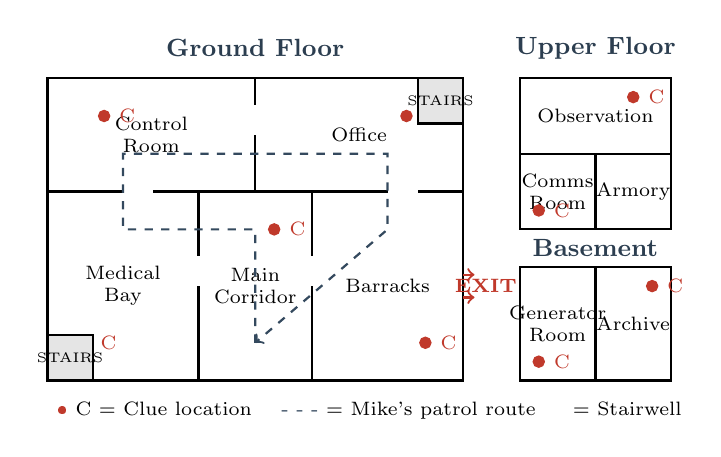
\begin{tikzpicture}[scale=0.48, every node/.style={font=\scriptsize}]
% --- Floor 1 (Ground) ---
\node[font=\small\bfseries, color=darkblue] at (5.5, 8.8) {Ground Floor};
% Outer walls
\draw[thick] (0,0) rectangle (11,8);
% Room divisions
\draw[thick] (4,0) -- (4,5);    % vertical wall
\draw[thick] (7,0) -- (7,5);    % vertical wall
\draw[thick] (0,5) -- (11,5);   % horizontal wall
\draw[thick] (5.5,5) -- (5.5,8); % upper vertical
% Doors (gaps in walls)
\draw[line width=2pt, white] (2,5) -- (2.8,5);
\draw[line width=2pt, white] (4,2.5) -- (4,3.3);
\draw[line width=2pt, white] (7,2.5) -- (7,3.3);
\draw[line width=2pt, white] (9,5) -- (9.8,5);
\draw[line width=2pt, white] (5.5,6.5) -- (5.5,7.3);
% Room labels
\node[align=center] at (2, 2.5) {Medical\\Bay};
\node[align=center] at (5.5, 2.5) {Main\\Corridor};
\node[align=center] at (9, 2.5) {Barracks};
\node[align=center] at (2.75, 6.5) {Control\\Room};
\node[align=center] at (8.25, 6.5) {Office};
% Clue markers
\filldraw[accentred] (1, 1) circle (0.15) node[right, xshift=2pt] {C};
\filldraw[accentred] (6, 4) circle (0.15) node[right, xshift=2pt] {C};
\filldraw[accentred] (10, 1) circle (0.15) node[right, xshift=2pt] {C};
\filldraw[accentred] (1.5, 7) circle (0.15) node[right, xshift=2pt] {C};
\filldraw[accentred] (9.5, 7) circle (0.15) node[right, xshift=2pt] {C};
% Patrol route (dashed)
\draw[mediumblue, thick, dashed, ->] (5.5, 1) -- (5.5, 4) -- (2, 4) -- (2, 6) -- (4.5, 6) -- (9, 6) -- (9, 4) -- (5.5, 1);
% Exit
\node[font=\scriptsize\bfseries, color=accentred] at (11.6, 2.5) {EXIT};
\draw[accentred, thick, ->] (11, 2.2) -- (11.3, 2.2);
\draw[accentred, thick, ->] (11, 2.8) -- (11.3, 2.8);
% Stairwells
\draw[thick, fill=gray!20] (0, 0) rectangle (1.2, 1.2);
\node at (0.6, 0.6) {\tiny STAIRS};
\draw[thick, fill=gray!20] (9.8, 6.8) rectangle (11, 8);
\node at (10.4, 7.4) {\tiny STAIRS};

% --- Floor labels ---
\node[font=\small\bfseries, color=darkblue] at (14.5, 8.8) {Upper Floor};
\draw[thick] (12.5,4) rectangle (16.5,8);
\draw[thick] (14.5,4) -- (14.5,6);
\draw[thick] (12.5,6) -- (16.5,6);
\node[align=center] at (13.5, 5) {Comms\\Room};
\node[align=center] at (15.5, 5) {Armory};
\node[align=center] at (14.5, 7) {Observation};
\filldraw[accentred] (13, 4.5) circle (0.15) node[right, xshift=2pt] {C};
\filldraw[accentred] (15.5, 7.5) circle (0.15) node[right, xshift=2pt] {C};

\node[font=\small\bfseries, color=darkblue] at (14.5, 3.5) {Basement};
\draw[thick] (12.5,0) rectangle (16.5,3);
\draw[thick] (14.5,0) -- (14.5,3);
\node[align=center] at (13.5, 1.5) {Generator\\Room};
\node[align=center] at (15.5, 1.5) {Archive};
\filldraw[accentred] (13, 0.5) circle (0.15) node[right, xshift=2pt] {C};
\filldraw[accentred] (16, 2.5) circle (0.15) node[right, xshift=2pt] {C};

% Legend
\node[font=\scriptsize, anchor=west] at (0, -0.8) {\textcolor{accentred}{\textbullet}\ C = Clue location \quad \textcolor{mediumblue}{- - -} = Mike's patrol route \quad \textcolor{gray}{$\blacksquare$} = Stairwell};
\end{tikzpicture}
\caption{Bunker floor plan showing room layout, clue placements, and patrol route across three floors.}
\end{figure}

Three playtesting sessions were conducted. Key findings: (1) initial sanity drain was too aggressive, preventing exploration past Floor 1; (2) Mike's patrol felt predictable, requiring randomized route switching; (3) players prioritized escaping over collecting clues until the clue-reading mechanic created enough narrative pull. Adjustments included reducing sanity drain, adding patrol randomization, rewarding Mike clues with small sanity restoration (+5 per clue), and implementing escalating chase speed after repeated detections. One playtester completed two runs in a single session, confirming the knowledge-based mastery hypothesis.

%===================================================================
\section{Technical Plan}
%===================================================================

\subsection{Technology Stack}

\begin{itemize}[leftmargin=2em, topsep=0pt, itemsep=2pt]
    \item \textbf{Engine:} Unity 6 with Universal Render Pipeline (URP)
    \item \textbf{Platform:} Windows (standalone .exe)
    \item \textbf{Rendering:} Volume-based post-processing for sanity effects (vignette, chromatic aberration, film grain, lens distortion)
    \item \textbf{AI:} Unity NavMesh for pathfinding; custom finite state machine for hunter behavior
    \item \textbf{Audio:} Unity 3D spatial audio for directional footstep tracking
    \item \textbf{Assets:} Abandoned Asylum (Unity Asset Store) for the bunker; Country House (Unity Asset Store) for the prologue
    \item \textbf{Version Control:} Git with Git LFS
\end{itemize}

\subsection{Team Roles and Schedule}

\begin{table}[h]
\centering
\small
\begin{tabular}{@{}p{3.5cm}p{4cm}p{5cm}@{}}
\toprule
\textbf{Team Member} & \textbf{Primary Role} & \textbf{Key Systems} \\
\midrule
Karl Seryani & Player Programmer & FP controller, interaction, clues, UI/HUD \\
\addlinespace
Kirill Delyukin & AI \& Audio Lead & Hunter AI, audio, sound design, endings \\
\addlinespace
Raghav Gulati & Environment \& VFX & Level design, lighting, sanity VFX, post-processing \\
\bottomrule
\end{tabular}
\end{table}

\begin{table}[h]
\centering
\small
\begin{tabular}{@{}p{3cm}p{4.5cm}p{5cm}@{}}
\toprule
\textbf{Week} & \textbf{Milestone} & \textbf{Key Deliverables} \\
\midrule
Feb 5 to 11 & Project Proposal & Deliverable 1 submission \\
Feb 12 to 18 & Foundation & FP controller, core architecture \\
Feb 19 to 25 & Core Mechanics & Flashlight, AI patrol, sanity \\
Feb 26 to Mar 4 & Gameplay Loop & Clues, AI chase, hiding \\
Mar 5 to 11 & Integration & Doors, search states, terminals \\
Mar 12 to 18 & Narrative + Polish & Clue placement, audio, HUD \\
Mar 19 to 25 & Build + Report & Deliverable 2 submission \\
Mar 26 to Apr 1 & Content Complete & All floors, endings, prologue \\
Apr 2 to 5 & Final Polish & Deliverable 3 + showcase video \\
\bottomrule
\end{tabular}
\end{table}

All team members collaborate on narrative writing, clue content, playtesting, and deliverable reports.

\end{document}
